\documentclass[12pt,
               a4paper,
               article,
               oneside,
               oldfontcommands,
               norsk]{memoir}
\makeatletter
\newcommand*{\rom}[1]{\expandafter\@slowromancap\romannumeral #1@}
\makeatother
\usepackage[utf8]{inputenc}
\usepackage{setspace}
\usepackage[T1]{fontenc}
\usepackage{titling}% the wheel somebody else kindly made for us earlier
\usepackage{fancyhdr}
\usepackage{tikz}
\usepackage{lmodern}
\usepackage{enumitem}
\usepackage{caption}
\usepackage{subcaption}
\usepackage{fancyvrb}
\usepackage[scaled]{beramono}
\usepackage[final]{microtype}
\usepackage{amssymb}
\usepackage{mathtools}
\usepackage{amsthm}
\usepackage{thmtools}
\usepackage{babel}
\usepackage{csquotes}
\usepackage{listings}
\lstset{basicstyle = \ttfamily}
\usepackage{float}
\usepackage{textcomp}
\usepackage{siunitx}
\usepackage{xcolor}
\usepackage{graphicx}
%\usepackage[colorlinks, allcolors = uiolink]{hyperref}
\usepackage[noabbrev]{cleveref}
\pretolerance = 2000
\tolerance    = 6000
\hbadness     = 6000
\newcounter{probnum}[section]
\newcounter{subprobnum}[probnum] 
\usepackage{dirtytalk}
\usepackage{listings}
\usepackage{xcolor}
\usepackage{caption}
\usepackage[section]{placeins}
\usepackage{varwidth}
\definecolor{uiolink}{HTML}{0B5A9D}
\definecolor{codegreen}{rgb}{0,0.6,0}
\definecolor{codegray}{rgb}{0.5,0.5,0.5}
\definecolor{codepurple}{rgb}{0.58,0,0.82}
\definecolor{backcolour}{rgb}{0.95,0.95,0.92}
\lstdefinestyle{mystyle}{
    backgroundcolor=\color{black},   
    commentstyle=\color{codegreen},
    keywordstyle=\color{magenta},
    numberstyle=\tiny\color{white},
    stringstyle=\color{codepurple},
    basicstyle=\ttfamily\footnotesize,
    breakatwhitespace=false,         
    breaklines=true,                 
    captionpos=b,                    
    keepspaces=true,                 
    numbers=left,                    
    numbersep=5pt,                  
    showspaces=false,                
    showstringspaces=false,
    showtabs=false,                  
    tabsize=3
}
\lstset{style=mystyle}
\usepackage{commath}
\usepackage[no-math]{fontspec}
%\setmainfont[Mapping=tex-text]{Chalkduster} 
\usepackage[defaultmathsizes]{mathastext}
\newtheorem{theorem}{Theorem}[section]
\newtheorem{corollary}{Corollary}[theorem]
\newcommand{\Q}{ \qquad \hfill \blacksquare}
\let\oldref\ref
\renewcommand{\ref}[1]{(\oldref{#1})}
\newtheorem{lemma}[theorem]{Lemma}
\pagecolor{darkgray}
\color{white}
\parindent 0ex
\pretitle{
	\begin{center}
		\rule[0.4pt]{300pt}{1.5pt} \\
			[0.10in]
\Huge}
		\title{STK1110}
\posttitle{\par\vskip0.3em{\scshape \textsc{ \large Obligatorisk oppgave 1}\\[-0.20in] \rule[0.4pt]{300pt}{1.5pt} \vspace{5mm}}
	\end{center}}
\author{Jonas Semprini Næss}
\begin{document}
\maketitle
NB! Kode på oppgave 1 f.) er skrevet i samarbeid med \say{erlek@math.uio.no}
\section*{Oppgave 0:}
a.) \\ 
Jeg tar STK1110 fordi jeg synes statistikk er viktig og det er et obligatorisk emne for den masteren jeg ønsker å søke meg inn på. I tillegg skal jeg videre ta STK2100 og da er det greit å ha tatt STK1110 fra før av.\\ 
b.) \\ 
Jeg forventer at STK1110 gir oss en god innføring i håndtering og modellering av data samt gir oss et godt teoretisk grunnlag til hvorfor vi kan praktiske statistikk som vi gjør. Men viktigst av alt så forventer jeg at kurset gir en interesse for faget så både fler og de som allerede tar kurset får sterke og nyttige verktøy å bruke i hverdagen samt fortsetter å se viktighet og anvendeligheten i statistikk.
\section*{Oppgave 1:}
a.) \emph{Vis at $E(X_i) = e^{\mu + \frac{\sigma^2}{2}}$ og at 
    $E(X_{i}^{2}) = e^{2\mu + 2\sigma^2}$ 
(Hint: du kan få bruk for momentgenererende funksjon for normalfordelingen 
$N(\mu, \sigma^2)$, som er $M_{Y}(t) = e^{\mu t+ \frac{1}{2} \sigma^2 t^2}$).}\vspace{3mm}\\
\textbf{Løsning:}\vspace{3mm}\\
Siden $Y$ er en normalfordelt variabel med forventning $\mu$ og varians $\sigma^2$ lønner det seg å analysere den momentgenererende funksjonen $M_{Y}(t)$ for å finne forventningen av den lognormalfordelte variablen $X$.\\
    Ved nærmere observasjon kan en således se at 
\begin{align*}
        M_{Y_i}(1) &= e^{\mu (1) + \frac{1}{2}\sigma^2(1)^2}\\[5pt]
                   &= e^{\mu + \frac{1}{2}\sigma^2}  \Q
\end{align*}
hvilket svarer til forventningen av $X_i$. For å finne forventningen av $X_{i}^2$ kan vi på lik måte analysere nte momente til $Y_i$.
\begin{align*}
E(X_{i}) = M_{Y_{i}}(1) \implies E(X_{i}^n) &= E((e^{Y_{i}})^n)\\[5pt]
&=
    M_{Y_{i}}(n)\\[5pt]
    &=
        e^{n\mu + n^2\frac{\sigma^2}{2}} 
\end{align*}
Som gir følgelig
\begin{align*}
    E(X_{i}^2) &= E((e^{Y_{i}})^2) \\[5pt]
               &= e^{2 \mu + 4 \frac{\sigma^2}{2}}\\[5pt]
               &= e^{2 \mu + 2 \sigma^2} \Q
\end{align*}
b.) \emph{Finn momentestimatorene $\hat{\mu}_{mom}$ og $\hat{\sigma^2}_{mom}$ for $\mu$ og $\sigma^2$, og beregn de tilsvarende estimatene for bilforsikringskravene.
}\vspace{3mm}\\
\textbf{Løsning:}\vspace{3mm}\\
Momentestimatorene til respektive parametere i en fordeling kan utrykkes ved å se på momentene til fordelingen. Ved å benytte oss av resultatene i a.) har vi 
\begin{align*} 
    E(X_i) = e^{\mu + \frac{\sigma^2}{2}}.  
\end{align*}
For å finne momentestimatoren til $\mu$ sammenligner vi dermed det teoretiske momente med det empiriske momente
\begin{align*}
    E(X_{i}) &= \frac{1}{n}\sum_{i=1}^{n} X_{i} \\[5pt]
    e^{\mu + \frac{\sigma^2}{2}} &= \frac{1}{n}\sum_{i=1}^{n} X_{i}
\end{align*}
tar så log på begge sider
\begin{align*}
    \mu + \frac{\hat{\sigma^2}}{2} = ln \left(\sum_{i=0}^{n} X_i \right) - ln(n) \\[5pt]
\end{align*}
og løser for $\hat{u}$
\begin{align}
    \label{eq1}
    \hat{\mu} = ln \left(\sum_{i=0}^{n} X_i \right) - ln(n) - \frac{\hat{\sigma^2}}{2}.
\end{align}
Videre ser vi på andre momente av $X_i$ for å finne $\hat{\sigma^2}$.
\begin{align*}
    E(X_{i}^2) &= \frac{1}{n} \sum_{i = 1}^{n} X_{i}^2 \\[7pt]
    e^{2\hat{\mu} + 2\hat{\sigma^2}} &= \frac{1}{n} \sum_{i = 1}^{n} X_{i}^2 \\[7pt]
    2\hat{\mu} + 2\hat{\sigma^2} &= ln \left( \sum_{i = 1}^{n} X_{i}^2 \right) - ln(n) \\[7pt]
\end{align*}
Løser igjen for $\hat{\mu}$
\begin{align}
    \label{eq2}
    \hat{\mu} = \frac{ln \left( \sum_{i = 1}^{n} X_{i}^2 \right) - ln(n)}{2} - \hat{\sigma^2}
\end{align}
og setter \ref{eq1} = \ref{eq2}
\begin{align*}
    ln \left(\sum_{i=0}^{n} X_i \right) - ln(n) - \frac{\hat{\sigma^2}}{2} &=  \frac{ln \left( \sum_{i = 1}^{n} X_{i}^2 \right) - ln(n)}{2} - \hat{\sigma^2}
\end{align*}
hvor vi sluttvis løser for $\hat{\sigma^2}$
\begin{align*}
\frac{\hat{\sigma^2}}{2} + ln \left(\sum_{i=0}^{n} X_i \right) &=  \frac{ln \left( \sum_{i = 1}^{n} X_{i}^2 \right)}{2} + ln(n)\\[7pt]
\hat{\sigma^2} &= ln \left( \sum_{i = 1}^{n} X_{i}^2 \right) - 2 ln \left(\sum_{i=0}^{n} X_i \right) + ln(n). \Q
\end{align*}
Herfra kan vi tilslutt løse for $\hat{\mu}$
\begin{align*}
    \hat{\mu} &= ln \left(\sum_{i=0}^{n} X_i \right) - ln(n) - \frac{\hat{\sigma^2}}{2}.\\[7pt]
    &= ln \left(\sum_{i=0}^{n} X_i \right) - ln(n) - \frac{ln \left( \sum_{i = 1}^{n} X_{i}^2 \right) - 2 ln \left(\sum_{i=0}^{n} X_i \right) + ln(n)}{2} \\[7pt]
    &= ln \left(\sum_{i=0}^{n} X_i \right) + ln \left(\sum_{i=0}^{n} X_i \right) - \frac{3}{2}ln(n) - \frac{ln \left( \sum_{i = 1}^{n} X_{i}^2 \right)}{2} \\[7pt]
    &= 2ln \left(\sum_{i=0}^{n} X_i \right) - \frac{3}{2}ln(n) - \frac{ln \left( \sum_{i = 1}^{n} X_{i}^2 \right)}{2}. \Q
\end{align*}
For å beregne estimatorene våre regner vi på datasettet i R. \vspace{4mm}\\
\begin{lstlisting}[language=R]
    forsikring.data = read.table("https://www.uio.no/studier/emner/matnat/math/STK1110/data/forsikringskrav.txt", header=T)

    forsikring = forsikring.data$X7.708

    mu_moment = round(2*log(sum(forsikring)) - (3/2)*(log(length(forsikring))) - (1/2)*(log(sum(forsikring^2))), 4)

    sigma_moment = log(sum(forsikring^2)) - 2*log(forsikring) + log(length(forsikring))
 \end{lstlisting}
Som gir verdiene for $\hat{\mu}$ og $\hat{\sigma^2}$
\begin{verbatim}
> mu_moment
[1] 2.7389
> sigma_moment
[1] 0.8901
\end{verbatim}
c.) \emph{Finn maksimum likelihood-estimatorene $\hat{\mu}_{mle}$ og $\hat{\sigma^2}_{mle}$ for $\mu$ og $\sigma^2$ på vanlig måte}\vspace{3mm}\\
\textbf{Løsning:}\vspace{3mm}\\
Ettersom verdiene i fordeling er uavhengig identisk fordelte vil vi kunne bruke det faktum at likelihoodfunksjonen er definert som produktet av sannsynlighetstetthetene til alle $X_{i}$. Siden $X_i$ er lognormalfordelt har den sannsynlighetsttethetsfunksjon
\begin{align*}
    f(x_1, \ldots, x_n; \mu, \sigma^2) = \frac{1}{x_i \sigma \sqrt{2 \pi}}e^{-\frac{(ln(x_i) - \mu)^2}{2 \sigma^2}}.
\end{align*}
likelihoodfunksjonen for $X_i$ er dermed definert som
\begin{align*}
    L(\mu, \sigma^2 \ | \ X_i ) &= \prod_{i=1}^{n}  f(x_1, \ldots, x_n; \mu, \sigma^2) \\[7pt]
                                &= \prod_{i=1}^{n} \frac{1}{X_i \sigma \sqrt{2 \pi}}e^{-\frac{(ln(X_i) - \mu)^2}{2 \sigma^2}}\\[7pt]
                                &= (2 \pi \sigma)^{-\frac{n}{2}} \prod_{i=1}^{n} \frac{1}{X_i} e^{-\frac{(ln(X_i) - \mu)^2}{2 \sigma^2}}
\end{align*}
Så tar vi logaritmen av denne som gir 
\begin{align*}
    \mathcal{L}(\mu, \sigma^2 \ | \ X_i) &= ln \left( (2 \pi \sigma^2)^{-\frac{n}{2}} \prod_{i=1}^{n} \frac{1}{X_i} e^{-\frac{(ln(X_i) - \mu)^2}{2 \sigma^2}} \right)\\[7pt]
    &= -\frac{n}{2} ln( 2 \pi \sigma^2 ) - ln \left( \sum_{i=1}^{n} X_i \right) -\frac{\sum_{i=1}^{n} (ln(X_i) - \mu)^2}{2 \sigma^2} \\[7pt]
    &= -\frac{n}{2} ln( 2 \pi \sigma^2 ) - ln \left( \sum_{i=1}^{n} X_i \right) - \frac{\sum_{i}^{n} ln(X_{i})^2}{2 \sigma^2} +  \frac{\sum_{i=1}^{n} ln(X_i) \mu}{\sigma^2} - \frac{n\mu^2}{2 \sigma^2}.\\[7pt]
\end{align*}
For å finne $\hat{\mu}_{mle}$ og $\hat{\sigma^2}_{mle}$ må vi partiellderivere $\mathcal{L}(\mu, \sigma^2 \ | \ X_i)$ med hensyn på de respektive parametrene og løse
\begin{align*}
    \frac{\partial \mathcal{L}}{\partial \mu} &= 0 \\[7pt]
    \frac{\partial \mathcal{L}}{\partial \sigma^2} &= 0
\end{align*}
som gir 
\begin{align*}
    \frac{\partial \mathcal{L}}{\partial \mu} &= \frac{\sum_{i=1}^{n} ln(X_i)}{\sigma^2} - \frac{n \mu}{\sigma^2} = 0 \\[7pt]
    \frac{n \mu}{\sigma^2} &= \frac{\sum_{i=1}^{n} ln(X_i)}{\sigma^2} \\[7pt]
    \hat{\mu}_{mle} &=  \frac{\sum_{i=1}^{n} ln(X_i)}{n}
\end{align*}
for $\mu$ og 
\begin{align*}
    \frac{\partial \mathcal{L}}{\partial \sigma^2} &= \frac{-n}{2 \sigma^2} - \left(- \frac{\sum_{i=1}^{n} (ln(X_i) - \mu)^2}{ 2 (\sigma^2)^2} \right) = 0 \\[7pt]
    \frac{n}{2\sigma^2} &=  \left(\frac{\sum_{i=1}^{n} (ln(X_i) - \mu)^2}{ 2 (\sigma^2)^2} \right) \\[7pt]
    \hat{\sigma^2}_{mle} &= \frac{\sum_{i = 1}^{n}(ln(X_i) - \hat{\mu}_{mle})^2}{n} \\[7pt]  
\end{align*}
setter vi inn for $\hat{\mu}_{mle}$ har vi sluttvis at 
\begin{align*}
    \hat{\sigma^2}_{mle} &= \frac{1}{n} \left(\sum_{i = 1}^{n}\left(ln(X_i)- \frac{\sum_{i=1}^{n}ln(X_i)}{n}\right)^2\right) \\[7pt].
\end{align*}
Beregner vi så maksimumestimatorene i R har vi at \vspace{4mm}\\
\begin{lstlisting}[language=R]
    forsikring.data = read.table("https://www.uio.no/studier/emner/matnat/math/STK1110/data/forsikringskrav.txt", header=T)

    forsikring = forsikring.data$X7.708

    u_mle = round((sum(log(forsikring)))/length(forsikring),4)

    sigma = sum((log(forsikring) - sum(log(forsikring))/length(forsikring))^2)

    sigma_mle = round(sigma/length(forsikring), 4)
\end{lstlisting}
\begin{verbatim}
> u_mle
[1] 2.7824
 > sigma_mle
[1] 0.7658
\end{verbatim}
hvor vi fra oppgave b ser at estimatorene er rimelig like, men med noen differanser. \vspace{5mm}\\
d.) \emph{Husk at $Y_i = log(X_i) \tilde N(\mu, \sigma^2), i = 1,\ldots,n$. Bruk dette, samt maksimum likelihood-estimatorene for parameterne i normalfordelingen (disse behøver
du ikke å utlede) til  å finne $\hat{\mu}_{mle}$ og $\hat{\sigma^2}_{mle}$ på en alternativ (og mye enklere) måte.
}\vspace{3mm}\\
\textbf{Løsning:}\vspace{3mm}\\
Vi vet at $Y_i = ln(X_i)$ er normalfordelt så vi kan skrive
\begin{align*}
    \mu = \bar{Y} = ln(\bar{X_i})
\end{align*}
hvor en kan skrive
\begin{align*}
    \bar{Y} = \frac{1}{n} \sum_{i=1}^{n} Y_i =  \frac{1}{n} \sum_{i=1}^{n} ln(X_i)
\end{align*}
hvilket hvis observerer fra c.) er det samme som 
\begin{align*}
    \hat{\mu}_{mle} = \frac{1}{n} \sum_{i=1}^{n} ln(X_i). \Q
\end{align*}
Likledes har vi for $\sigma^2$ at
\begin{align*}
    \sigma^2 = \frac{1}{n} \sum_{i=1}^{n} (Y_i - \bar{Y})^2
\end{align*}
hvilket hvis vi setter inn for $Y_i$ og $\bar{Y}$ gir 
\begin{align*}
\hat{\sigma^2} = \frac{1}{n} \left(\sum_{i = 1}^{n}\left(ln(X_i)- \frac{\sum_{i=1}^{n}ln(X_i)}{n}\right)^2\right) \Q
\end{align*}
som er det samme som $\hat{\sigma^2}_{mle}$.\vspace{5mm}\\
e.) \emph{Vis at informasjonsmatrisa for èn observasjon er gitt ved} 
\begin{align*}
    I(\mu, \sigma^2) = 
\begin{pmatrix}
    \frac{1}{\sigma^2} & 0\\[3pt]
    0 & \frac{1}{2 \sigma^4}
\end{pmatrix}
\end{align*}
\textbf{Løsning:}\vspace{3mm}\\
Informasjonselemente i Fishermatrisen for én observasjon er gitt ved Hesse-matrisen
\begin{align*}
    I(\mu, \sigma^2) = 
    \begin{pmatrix}
        -E \left(\frac{\partial^2 ln(f(x_1, \ldots, x_n; \mu, \sigma^2))}{\partial^2 \mu} \right) & -E \left( \frac{\partial^2 ln(f(x_1, \ldots, x_n; \mu, \sigma^2))}{\partial \mu \partial \sigma^2} \right) \\[5pt]
       -E \left(\frac{\partial^2 ln(f(x_1, \ldots, x_n; \mu, \sigma^2))}{\partial \sigma^2 \partial u} \right) & -E \left( \frac{\partial^2 ln(f(x_1, \ldots, x_n; \mu, \sigma^2))}{\partial (\sigma^2)^2} \right)
    \end{pmatrix}
\end{align*}
Starter vi med å ta den andre ordens partiellderiverte av $\mu$ gir det
\begin{align*}
    \frac{\partial ln(f(x_1, \ldots, x_n; \mu, \sigma^2))}{\partial \mu} &= \frac{\partial}{\partial \mu} - \left( \frac{ln(X_i)^2 - 2ln(X_i)\mu + \mu^2}{2 \sigma^2}\right) - ln(\sqrt{2 \pi} x \sigma) \\[7pt]
    &= - \frac{1}{\sigma^2} \left(- ln(X_i) + \mu \right) \\[7pt]
    \frac{\partial^2 ln(f(x_1, \ldots, x_n; \mu, \sigma^2))}{\partial^2 \mu} &= - \frac{1}{\sigma^2}
\end{align*}
og sluttvis har vi
\begin{align*}
    -E \left(\frac{\partial^2 ln(f(x_1, \ldots, x_n; \mu, \sigma^2))}{\partial^2 \mu} \right) &= -E(- \frac{1}{\sigma^2})\\[7pt]
                        &= \frac{1}{\sigma^2}.
\end{align*}
Følger vi samme regime for $\sigma^2$ har vi 
\begin{align*}
    \frac{\partial ln(f(x_1, \ldots, x_n; \mu, \sigma^2))}{\partial u} &= \frac{1}{2} \left( \frac{(ln(X_i) - \mu)^2}{u^2} \right) + \frac{1}{2\sqrt{u}}\frac{1}{\sqrt{u}} \qquad ; \qquad \boxed{u = \sigma^2} \\[7pt]
    &= \frac{1}{2} \left( \frac{(ln(X_i) - \mu)^2}{u} \right) - \frac{1}{2u} \\[7pt]
    \frac{\partial^2 ln(f(x_1, \ldots, x_n; \mu, \sigma^2))}{\partial^2 u}&= -\frac{1}{4} \left( \frac{(ln(X_i) - \mu)^2}{u^3} \right)  - \frac{1}{2u^2} \\[7pt]
    \frac{\partial^2 ln(f(x_1, \ldots, x_n; \mu, \sigma^2))}{\partial (\sigma^2)^2}&= -\frac{1}{4} \left( \frac{(ln(X_i) - \mu)^2}{\sigma^6} \right)  - \frac{1}{2\sigma^4} \\[7pt]
\end{align*}
som gir 
\begin{align*}
    -E\left(-\frac{1}{4} \left( \frac{(ln(X_i) - \mu)^2}{\sigma^6} \right) - \frac{1}{2\sigma^4} \right) &=  -E\left(-\frac{1}{4} \left( \frac{(ln(X_i) - \mu)^2}{\sigma^6} \right) \right) - E\left( - \frac{1}{2\sigma^4} \right) \\[7pt]
    &= 0 + \frac{1}{2 \sigma^4} \\[7pt]
    & = \frac{1}{2 \sigma^4}.
\end{align*}
Og sluttvis har vi for de førsteordens partiellderiverte respektive parametrene
\begin{align*}
    \frac{\partial^2 ln(f(x_1, \ldots, x_n; \mu, \sigma^2))}{\partial \mu \partial \sigma^2} &= \frac{\ln(X_i)}{\sigma^2} - \frac{\mu}{\sigma^2} \\[7pt]
    &= \frac{\ln(X_i) - \mu}{\sigma^2}
\end{align*}
hvor den negative forventningen gir 
\begin{align*}
    -E \left(\frac{\partial^2 ln(f(x_1, \ldots, x_n; \mu, \sigma^2))}{\partial \mu \partial \sigma^2} \right) &= -E \left( \frac{\ln(X_i) - \mu}{\sigma^2} \right) \\[7pt]
    &= \frac{\mu}{\sigma^2} - E \left( \frac{ln(X_i)}{\sigma^2}\right) \\[7pt]
    &= \frac{\mu}{\sigma^2} - \frac{\mu}{\sigma^2} \\[7pt]
    &= 0
\end{align*}
og setter vi sammen resultatene har vi at 
\begin{align*}
    I(\mu, \sigma^2) = 
    \begin{pmatrix}
        -E \left(\frac{\partial^2 ln(f(x_1, \ldots, x_n; \mu, \sigma^2))}{\partial^2 \mu} \right) & -E \left( \frac{\partial^2 ln(f(x_1, \ldots, x_n; \mu, \sigma^2))}{\partial \mu \partial \sigma^2} \right) \\[5pt]
       -E \left(\frac{\partial^2 ln(f(x_1, \ldots, x_n; \mu, \sigma^2))}{\partial \sigma^2 \partial u} \right) & -E \left( \frac{\partial^2 ln(f(x_1, \ldots, x_n; \mu, \sigma^2))}{\partial (\sigma^2)^2} \right)
    \end{pmatrix}
    = 
    \begin{pmatrix}
        \frac{1}{\sigma^2} & 0\\[3pt]
        0 & \frac{1}{2 \sigma^4}
    \end{pmatrix} \Q
\end{align*}
som var det vi skulle vise. Standardfeilen til informasjonsmatrisen er gitt ved å ta kvadratroten til diagonalelementene i den inverse Fishermatrisen. Da har vi 
\begin{align*}
    I(\mu, \sigma^2)^{-1} &= \frac{1}{\frac{1}{2 \sigma^6}} 
    \begin{pmatrix}
        \frac{1}{\sigma^2} & 0\\[3pt]
        0 & \frac{1}{2 \sigma^4}
    \end{pmatrix}\\[7pt]
    &=  \begin{pmatrix}
       \sigma^2 & 0\\[3pt]
        0 & 2 \sigma^4
    \end{pmatrix}
\end{align*}
og $SD(\mu, \sigma^2) = \sigma, \sqrt{2}\sigma^2$. \vspace{4mm}\\ 
f.) \emph{Estimer nå standardfeilen til $\hat{\mu}_{mle}$ og $\sigma^2_{mle}$ for foriskringsdataene ved hjelp av ikke-parametrisk bootstrapping. Sammenlign med estimatene du fikk i e) og kommenter.
}\vspace{3mm}\\
\textbf{Løsning:}\vspace{3mm}\\
Vi løser oppgaven ved hjelp av følgende R-script \vspace{4mm}\\
\begin{lstlisting}[language=R]
    bilforsikring.krav = read.table("https://www.uio.no/studier/emner/matnat/math/STK1110/data/forsikringskrav.txt")
    n = length(bilforsikring.krav$V1)
    
    iterations = 1000
    arr_mu_mle = rep(0,iterations)
    arr_sigma_2_mle = rep(0,iterations)
    
    for (i in 1:iterations){
     temp = sample(bilforsikring.krav$V1, replace=T)  
     mu_mle = sum(log(temp))/n
     sigma_2_mle = sum((log(temp) - mu_mle)^2)/n 
     
     arr_mu_mle[i] = mu_mle
     arr_sigma_2_mle[i] = sigma_2_mle
    }
    
    sd_mu_mle_boot = sd(arr_mu_mle)*sqrt(n)
    sd_sigma_2_mle_boot = sd(arr_sigma_2_mle)*sqrt(n)
    
    sigma = sd(log(bilforsikring.krav$V1))
    
    sd_mu_mle = sigma^2
    sd_sigma_2_mle = 2*sigma^4
    
    abs(sd_mu_mle - sd_mu_mle_boot)
    abs(sd_sigma_2_mle - sd_sigma_2_mle_boot)
\end{lstlisting}
som gir oss verdiene 
\begin{verbatim}
> sd_mu_mle_boot
[1] 0.9104013

> sd_sigma_2_mle_boot
[1] 1.1427

> sigma
[1] 0.875151

> sd_mu_mle
[1] 0.7658893

> sd_sigma_2_mle
[1] 1.173173

> abs(sd_mu_mle - sd_mu_mle_boot)
[1] 0.144512

> abs(sd_sigma_2_mle - sd_sigma_2_mle_boot)
[1] 0.03047338
\end{verbatim}
hvor vi observerer at estimatorene våre fra maksimumlikelihoodfunksjonen er ganske gode sammenlignet med standardavviket fra informasjonsmatrisen. \vspace{4mm}\\

g.) \emph{Fra a) vet vi at $ \phi = E(Xi) = e^{\mu + \frac{\sigma^2}{2}} = \phi(\mu,\sigma^2)$. Hva er maksimum likelihood-estimatoren $\hat{\phi}_{mle}$ for $\phi$? Beregn det estimatet for bilforsikringskravene. En alternativ estimator for $\phi$ er den forventningsrette $\bar{X} = \sum_{i=1}^{n} X_i$. Beregn estimatet $\bar{x}$ for forsikringsdataene og sammenlign med maksimum likelihood-estimatet.
}\vspace{3mm}\\
\textbf{Løsning:}\vspace{3mm}\\
Vi vet at $ E(Xi) = e^{\mu + \frac{\sigma^2}{2}}$ og ønsker vi å finne maksimumlikelihoodestimatoren av $E(X_i)$ kan vi simpelthen sette inn estimatore våre fra tidligere 
\begin{align*}
    \hat{E(X_i)}_{mle} &= e^{\hat{\mu}_{mle} + \frac{\hat{\sigma}_{mle}}{2}} \\[7pt]
    &= e^{\frac{\sum_{i=1}^{n} ln(X_i)}{n} + \frac{1}{2n} \left(\sum_{i = 1}^{n}\left(ln(X_i)- \frac{\sum_{i=1}^{n}ln(X_i)}{n}\right)^2\right)}
\end{align*}
og sammenligne med den forventingsrette estimatoren $\bar{X}$. Dette kan løses ved følgende R-script \vspace{4mm}\\ 
\begin{lstlisting}[language=R]
forsikring.data = read.table("https://www.uio.no/studier/emner/matnat/math/STK1110/data/forsikringskrav.txt", header=T)

forsikring = forsikring.data$X7.708

u_mle = round((sum(log(forsikring)))/length(forsikring),4)

sigma = sum((log(forsikring) - sum(log(forsikring))/length(forsikring))^2)

sigma_mle = round(sigma/length(forsikring), 4)

forventing_mle = round(exp(u_mle + (1/2)*sigma_mle),4)

X_strek = round(sum(forsikring)/length(forsikring),4)
\end{lstlisting}
som gir følgende verdier 
\begin{verbatim}
> forventing_mle
[1] 23.6959

> X_strek
[1] 24.141
\end{verbatim}
hvilket viser at likelihoodestimatoren gir en ganske god estimering.
\section*{Oppgave 2:}
a.) \emph{$E(X_i)$ og $V(X_i)$}
\vspace{3mm}\\
\textbf{Løsning:}\vspace{3mm}\\
For en kontinuerlig sannsynlighetstetthetfunksjon har vi at 
\begin{align*}
    E(X) = \int_{-\infty}^{\infty} xf(x) \ dx 
\end{align*}
bruker vi dette for den uniforme sannsynlighetsfordelingen gir det 
\begin{align*}
    E(X_i) &= \int_{-\infty}^{\infty} xf(x) \ dx \\[7pt]
    &= \underbrace{\int_{-\infty}^{0} xf(x) \ dx}_{ 0} + \int_{0}^{\theta} xf(x) \ dx \\[7pt]
    &= \int_{0}^{\theta} x \frac{1}{\theta} \ dx \\[7pt]
    &=  \frac{1}{\theta} \left[ {\frac{x^2}{2}}\right]_{0}^{\theta} \\[7pt]
    &= \frac{\theta}{2}.
\end{align*}
Videre husker vi at $Var(X_i) = E(X_i^2) - (E(X_i))^2$ og for å kunne gå videre må vi beregne $E(X_i^2)$. 
\begin{align*}
    E(X_{i}^2) &= \int_{0}^{\theta} x^2 \frac{1}{\theta} \ dx \\[7pt]
    &= \frac{1}{\theta} \left[ {\frac{x^3}{3}}\right]_{0}^{\theta} \\[7pt]
    &= \frac{\theta^2}{3}.
\end{align*}
Da har vi at 
\begin{align*}
Var(X_i) &= E(X_i^2) - (E(X_i))^2 \\[7pt]
&= \frac{\theta^2}{3} - \frac{\theta^2}{4}\\[7pt]
&=\frac{\theta^2}{12}.
\end{align*}
b.) \emph{Vis at momentestimatoren for $\theta$ er $\hat{\theta}_{mom} = 2\bar{X}$. Er estimatoren forvent-
ningsrett?}
\vspace{3mm}\\
\textbf{Løsning:}\vspace{3mm}\\
Vi vet at $\bar{X} = \frac{1}{n} \sum_{i=1}^{n} X_i$ og $E(X_i) = \frac{\theta}{2}$. Bruker vi denne informasjonen har vi
\begin{align*}
    E(X_i) &= \bar{X} \\[7pt]
    \frac{\theta}{2} &= \frac{1}{n} \sum_{i=1}^{n} X_i \\[7pt]
    \hat{\theta}_{mom} & = 2 \left(\frac{1}{n} \sum_{i=1}^{n} X_i \right) \\[7pt]
    \hat{\theta}_{mom} &= 2 \bar{X}
\end{align*}
hvor vi ser at
\begin{align*}
    E(\hat{\theta}_{mom}) = 2 E(\bar{X}) = 2 \frac{\theta}{2} = \theta
\end{align*}
$\hat{\theta}_{mom}$ er forventningsrett. \vspace{4mm}\\
c.)  \emph{Bestem standardfeilen til $\hat{\theta}_{mom}$.}
\vspace{3mm}\\
\textbf{Løsning:}\vspace{3mm}\\
Standardfeilen til estimatoren $\hat{\theta}_{mom}$ er det samme som standardavviket til estimatoren. Det betyr at
\begin{align*}
    SD(\hat{\theta}_{mom}) &= \sqrt{Var(\hat{\theta}_{mom})} \\[7pt]
    &= \sqrt{E(\hat{\theta}_{mom}^2) - (E(\hat{\theta}_{mom}))^2}\\[7pt]
    &= \sqrt{E(4 \bar{X}) - \theta^2} \\[7pt]
    &= \sqrt{\frac{4\theta^2}{3} - \frac{3 \theta^2}{3}} \\[7pt]
    &= \sqrt{\frac{\theta^2}{3}} \\[7pt]
    &= \frac{\sqrt{3}\theta}{3}.
\end{align*}
d.) \emph{Vis at likelihooden er gitt ved}
\begin{align*}
    f(x_1, \ldots, x_n; \theta) =
    \begin{cases}
    \frac{1}{\theta^n}, \ 0 \leq x \leq \theta \\[4pt]
    0 , \ \text{ellers}
    \end{cases}
\end{align*}
\emph{og forklar at maksimum likelihood-estimatoren for $\theta$ er $\hat{\theta}_{mle} = max(X_i)$}
\vspace{3mm}\\
\textbf{Løsning:}\vspace{3mm}\\
Vi husker fra oppgave 1 c.) at likelihoodfunksjonen er gitt ved
\begin{align*}
    L(\theta | X_i) &= \prod_{i=1}^{n} f(x_1, \ldots, x_n; \theta) \\[7pt]
    &= \prod_{i=1}^{n} \frac{1}{\theta} \\[7pt]
    &= \frac{1}{\theta^n} \Q
\end{align*}
Når vi skal finne maksimumlikelihoodestimatoren til $\theta$ hjelper det å se på hvordan likelihoodfunksjonen utvikler seg.
Selve funksjonen $\frac{1}{\theta^n}$ er strengt avtakende for $\theta \geq x_n$ og maksimert hvis $x_n = \theta$ jmf. $[0 \leq x \leq \theta]$. For $x_n \geq \theta$ er funksjonen udefinert.
Dermed må maksimumlikelihoodestimatoren være $max(X_i)$.\vspace{4mm}\\
e.) \emph{Det kan vises at forventningen og andremomentet til $\hat{\theta}_{mle}$ er henholdsvis}
\begin{align*}
    E(\hat{\theta}_{mle}) = \frac{n\theta}{n+1} \ \text{og} \ E(\hat{\theta}_{mle}^2) = \frac{n\theta^2}{n+2}
\end{align*}
\emph{hvilket betyr at $\hat{\theta}_{mle}$ ikke er forventningsrett for $\theta$. Bruk resultatene over
til å vise at estimatoren $\tilde{\theta} = \frac{n+1}{n}\hat{\theta}_{mle}$ er forventningsrett og til å finne standardfeilen til $\tilde{\theta}$.}
\vspace{3mm}\\
\textbf{Løsning:}\vspace{3mm}\\
Vi har at 
\begin{align*}
    E(\tilde{\theta}) &= E \left(\frac{n+1}{n} \hat{\theta}_{mle} \right)\\[7pt]
    &= \frac{n+1}{n} E(\hat{\theta}) \\[7pt]
    &=  \frac{n+1}{n} \frac{n\theta}{n+1} \\[7pt]
    &= \theta \Q.
\end{align*}
Standardavviket beregnes på samme måte som tidligere 
\begin{align*}
    Var(\tilde{\theta}) &= E(\tilde{\theta}^2) - (E(\tilde{\theta}))^2 \\[7pt]
    &= E\left(\left(\frac{n + 1}{n}\right)^2 \hat{\theta}^2\right) - \theta^2 \\[7pt]
    &= \frac{(n+1)^2}{n^2} \frac{n\theta^2}{n+2} - \theta^2 \\[7pt]
    &= \frac{\theta^2}{n(n+2)} \\[7pt]
    SD(\tilde{\theta}) &= \frac{\theta}{\sqrt{n(n +2)}}
\end{align*}
f.) \emph{Sammenlign momentestimatoren $\hat{\theta}_{mom}$ fra b) med $\tilde{\theta}$. Hvilken estimator vel-
ger du? Svaret skal begrunnes.}
\vspace{3mm}\\
\textbf{Løsning:}\vspace{3mm}\\
For å sammenligne estimatorene ser vi på standarfeilen til begge to, nemlig 
\begin{align*}
    SD(\tilde{\theta}) &= \frac{\theta}{\sqrt{n(n+2)}} \\[7pt]
    SD(\hat{\theta}_{mom}) &= \frac{\sqrt{3} \theta}{3}
\end{align*}
Siden standardfeilen til $\tilde{\theta}$ varierer med $n$ er det verdt å sjekke når denne vil bli mindre enn standarfeilien til $\hat{\theta}_{mom}$.
\begin{align*}
    n(n+2) > 3 \\[7pt]
    n^2 + 2n > 3  \\[7pt]
    n^2 + 2n - 3 > 0 \\[7pt]
    (n + 3)(n-1) > 0
\end{align*}
Siden $n$ ikke kan være negativ (ville gitt et komplekst tall) må $n > 1$ for at $\tilde{\theta}$ skal være en bedre estimator. Derfor ville jeg heller valgt $\tilde{\theta}$ enn $\hat{\theta}_{mom}$ siden standardfeilen er konstant og veldig mye dårligere for større $n$.
g.) \emph{Sjekk hvordan teorien virker i praksis ved å simulere $n = 20$ observasjoner fra uniform fordeling på $[0,1]$ (du kan bruke data = runif(20) i R). I dette tilfellet er den sanne verdien for $\theta$ lik 1. Hvor nær kommer du med de to es- timatorene du sammenlignet i forrige punkt? Gjenta prosedyren over mange ganger (f.eks. 1000 til sammen) for å illustrere poenget i f), og presenter resultatene grafisk (f.eks. i et boksplott eller et histogram).}
\vspace{3mm}\\
\textbf{Løsning:}\vspace{3mm}\\
Kan løse oppgaven ved følgende R-script
\begin{lstlisting}[language=R]
    n = 1000

    uni = runif(n)

    sd_theta_tilde = 1/(sqrt(n*(n+2)))

    sd_theta_hat = (sqrt(3)*1)/3

    pdf(file="estimatorer.pdf")

    hist(sd_theta_tilde, breaks = "Sturges")

    hist(sd_theta_hat, breaks = "Sturges")

    dev.off()
    \end{lstlisting}
hvor tisvarende verdier er 
\begin{verbatim}
> sd_theta_hat
[1] 0.5773503

> sd_theta_tilde
[1] 0.0009990015
\end{verbatim}
hvor vi ut i fra teorien ser at det stemmer ganske godt hvilken estimator som er ideel. Ett mulig plot av standardavvikene kan vises i dette histogrammet.
\begin{figure}[H]
	\centering
	\begin{subfigure}[H]{0.8\textwidth}
	\centering
	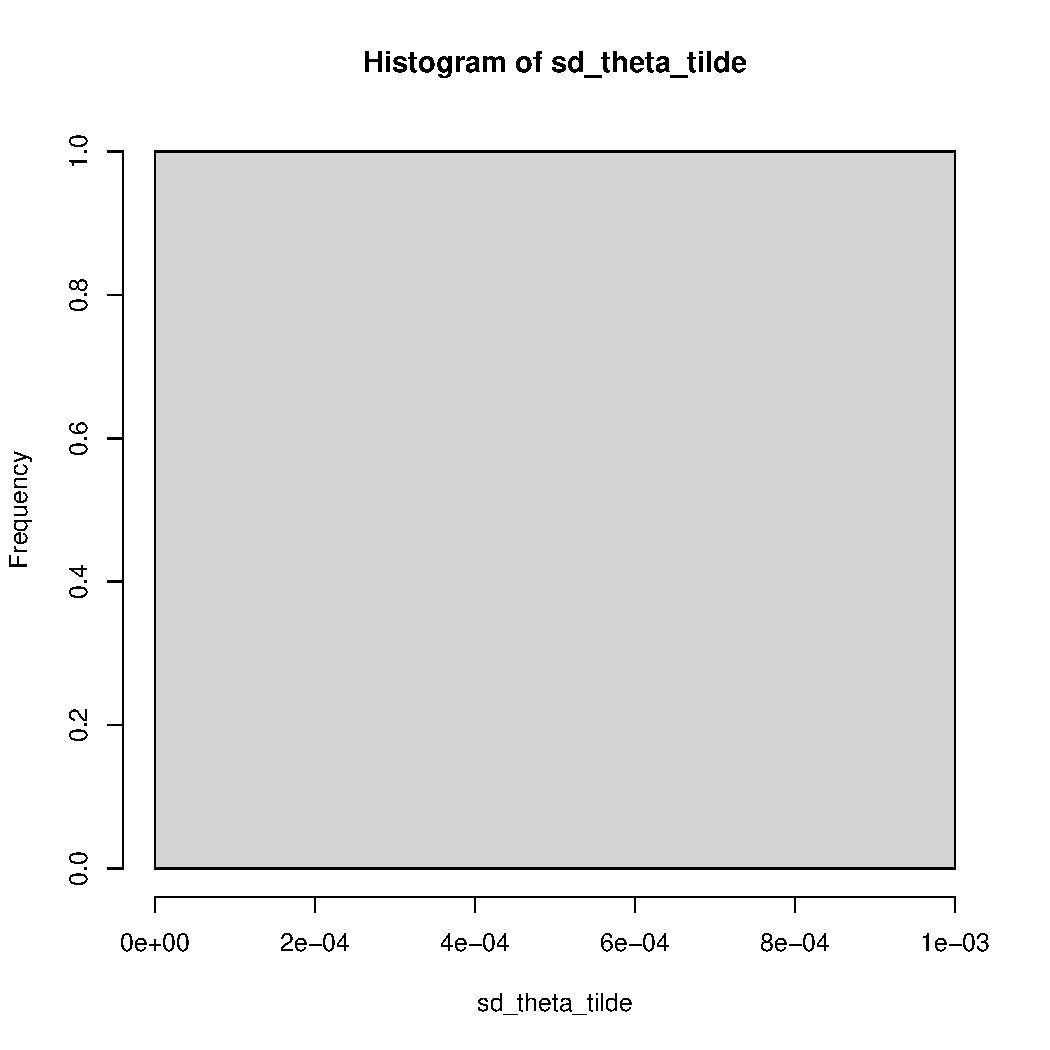
\includegraphics[width=\textwidth]{estimatorer.pdf}
	\end{subfigure}
	\vfill
	\begin{subfigure}[H]{0.8\textwidth}
	\centering
	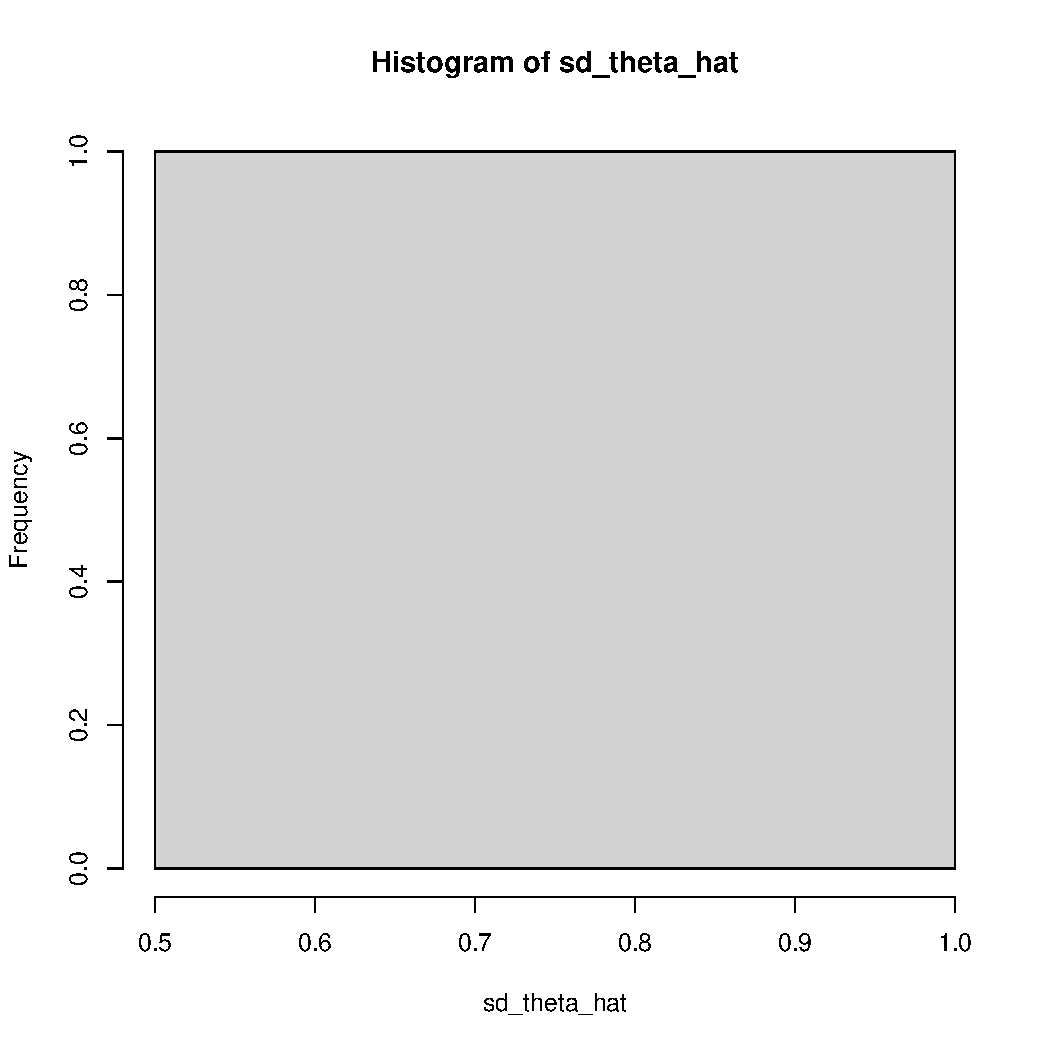
\includegraphics[width=\textwidth]{estimatorer1.pdf} 
	\end{subfigure}
\end{figure}
\end{document} 